% !TEX root = ../main.tex

\section{Experimental Evaluation}
\label{sec:experiments}
% ==================================================

% Keep the project macro from swallowing spaces in this and following sections.
\makeatletter
\renewcommand{\HVM}{HVM-Codec\futurelet\@let@token\HVM@space}
\newcommand{\HVM@space}{%
  \ifx\@let@token\bgroup\else
  \ifx\@let@token,\else
  \ifx\@let@token.\else
  \ifx\@let@token;\else
  \ifx\@let@token:\else
  \ifx\@let@token)\else
  \ifx\@let@token]\else
  \space
  \fi\fi\fi\fi\fi\fi\fi}
\makeatother

\subsection{Experimental Setup}
\label{subsec:exp_setup}

The evaluation uses three types of sequences: NCD, TUM, and GDUT. NCD and TUM provide public benchmark sequences, while GDUT contains real robot data collected in our deployment environment. This combination allows the experiments to cover both standard datasets and robot-captured visual streams under the same \HVM{} evaluation protocol.

All experiments follow a unified prepare--encode--decode--eval pipeline. The preparation stage organizes image sequences and trajectory references; the encoder converts dense frames into the transmitted \HVM{} representation; the decoder produces a generated visual sequence from the image--text memory; and the evaluation stage runs the VSLAM backend on both original and generated sequences. Unless otherwise stated, phase correlation (PC) is used as the default lightweight motion estimator on the edge side. The cloud side uses an image--text conditioned world-model decoder, with Base and LoRA variants compared in the ablation study.

Trajectory quality is measured from the VSLAM backend output using evo after Sim(3) alignment, and the reported task metric is APE RMSE. Compression is measured by comparing the size of the original image sequence with the size of the transmitted \HVM{} representation. LPIPS, SSIM, and FID are used only as auxiliary image-fidelity metrics in the LoRA ablation; they are not the final task-level objective of \HVM.

\subsection{End-to-End Compression and VSLAM Accuracy}
\label{subsec:compression_accuracy}

The first experiment evaluates end-to-end transmission reduction and VSLAM trajectory accuracy across nine test fragments.

% This table is included by sections/04_experiments.tex.
\begin{table*}[!t]
\renewcommand{\arraystretch}{1.14}
\caption{End-to-end compression and VSLAM trajectory accuracy with GT path-length context.}
\label{tab:compression_accuracy}
\centering
\footnotesize
\setlength{\tabcolsep}{2pt}
\begin{tabular*}{\textwidth}{@{\extracolsep{\fill}}cc*{8}{c}@{}}
\toprule
\multirow{2}{*}{Dataset} & \multirow{2}{*}{Seq.} & \multirow{2}{*}{$L_{\mathrm{GT}}$ (m)} & \multicolumn{3}{c}{Payload} & \multicolumn{3}{c}{APE RMSE} & \multirow{2}{*}{$|\Delta|/L_{\mathrm{GT}}$ (\%)} \\
\cmidrule(lr){4-6}\cmidrule(lr){7-9}
 & & & Raw (MiB) & VLMem (MiB) & Red. (\%) & ORI (m) & REC (m) & $\Delta$ (m) & \\
\midrule
\multirow{4}{*}{NCD} & 1 & 16.80 & 170.66 & \textbf{4.99} & \textbf{97.1} & 0.071 & 0.102 & +0.031 & 0.185 \\
 & 2 & 42.74 & 259.48 & \textbf{9.04} & \textbf{96.5} & 0.142 & 0.286 & +0.144 & 0.337 \\
 & 3 & 64.19 & 378.03 & \textbf{14.01} & \textbf{96.3} & 0.320 & 0.585 & +0.265 & 0.413 \\
 & Avg. & 41.24 & 269.39 & \textbf{9.35} & \textbf{96.6} & 0.178 & 0.324 & +0.147 & 0.311 \\
\midrule
\multirow{4}{*}{TUM} & 1 & 2.72 & 130.89 & \textbf{5.94} & \textbf{95.5} & 0.150 & 0.220 & +0.074 & 2.721 \\
 & 2 & 5.94 & 263.21 & \textbf{11.00} & \textbf{95.8} & 0.224 & \textbf{0.187} & -0.037 & 0.623 \\
 & 3 & 12.68 & 518.74 & \textbf{21.25} & \textbf{95.9} & 1.129 & \textbf{1.062} & -0.067 & 0.528 \\
 & Avg. & 7.11 & 304.28 & \textbf{12.73} & \textbf{95.7} & 0.501 & \textbf{0.490} & -0.010 & 1.291 \\
\midrule
\multirow{4}{*}{GDUT} & 1 & 20.89 & 268.93 & \textbf{5.52} & \textbf{97.9} & 0.351 & 0.454 & +0.103 & 0.493 \\
 & 2 & 41.22 & 547.55 & \textbf{10.81} & \textbf{98.0} & 1.994 & \textbf{1.162} & -0.832 & 2.018 \\
 & 3 & 84.84 & 1093.29 & \textbf{16.97} & \textbf{98.4} & 1.901 & 2.553 & +0.652 & 0.769 \\
 & Avg. & 48.98 & 636.59 & \textbf{11.10} & \textbf{98.1} & 1.415 & \textbf{1.390} & -0.026 & 1.093 \\
\midrule
Overall & Avg. & 32.45 & 403.42 & \textbf{11.06} & \textbf{96.8} & 0.698 & 0.735 & +0.037 & 0.898 \\
\bottomrule
\end{tabular*}%
\par\vspace{2pt}
\parbox{\textwidth}{\emph{Note:} $L_{\mathrm{GT}}$ is the GT path length. ORI and REC denote VSLAM results from original and reconstructed frames, respectively. $\Delta\mathrm{APE}=\mathrm{APE}_{\mathrm{REC}}-\mathrm{APE}_{\mathrm{ORI}}$ is signed, and $|\Delta|/L_{\mathrm{GT}}$ is a path-normalized deviation. Average rows are arithmetic means over sequence rows; normalized averages are computed from sequence-wise normalized deviations. Bold values in the VLMem and reduction columns highlight the compact transmitted payload and the corresponding transmission reduction. Bold REC APE values indicate cases where the reconstructed sequence obtains lower aligned APE RMSE than the original sequence. Negative $\Delta$APE indicates lower aligned REC APE RMSE, not physically superior reconstructed observations.}
\end{table*}


\begin{figure*}[!t]
\centering
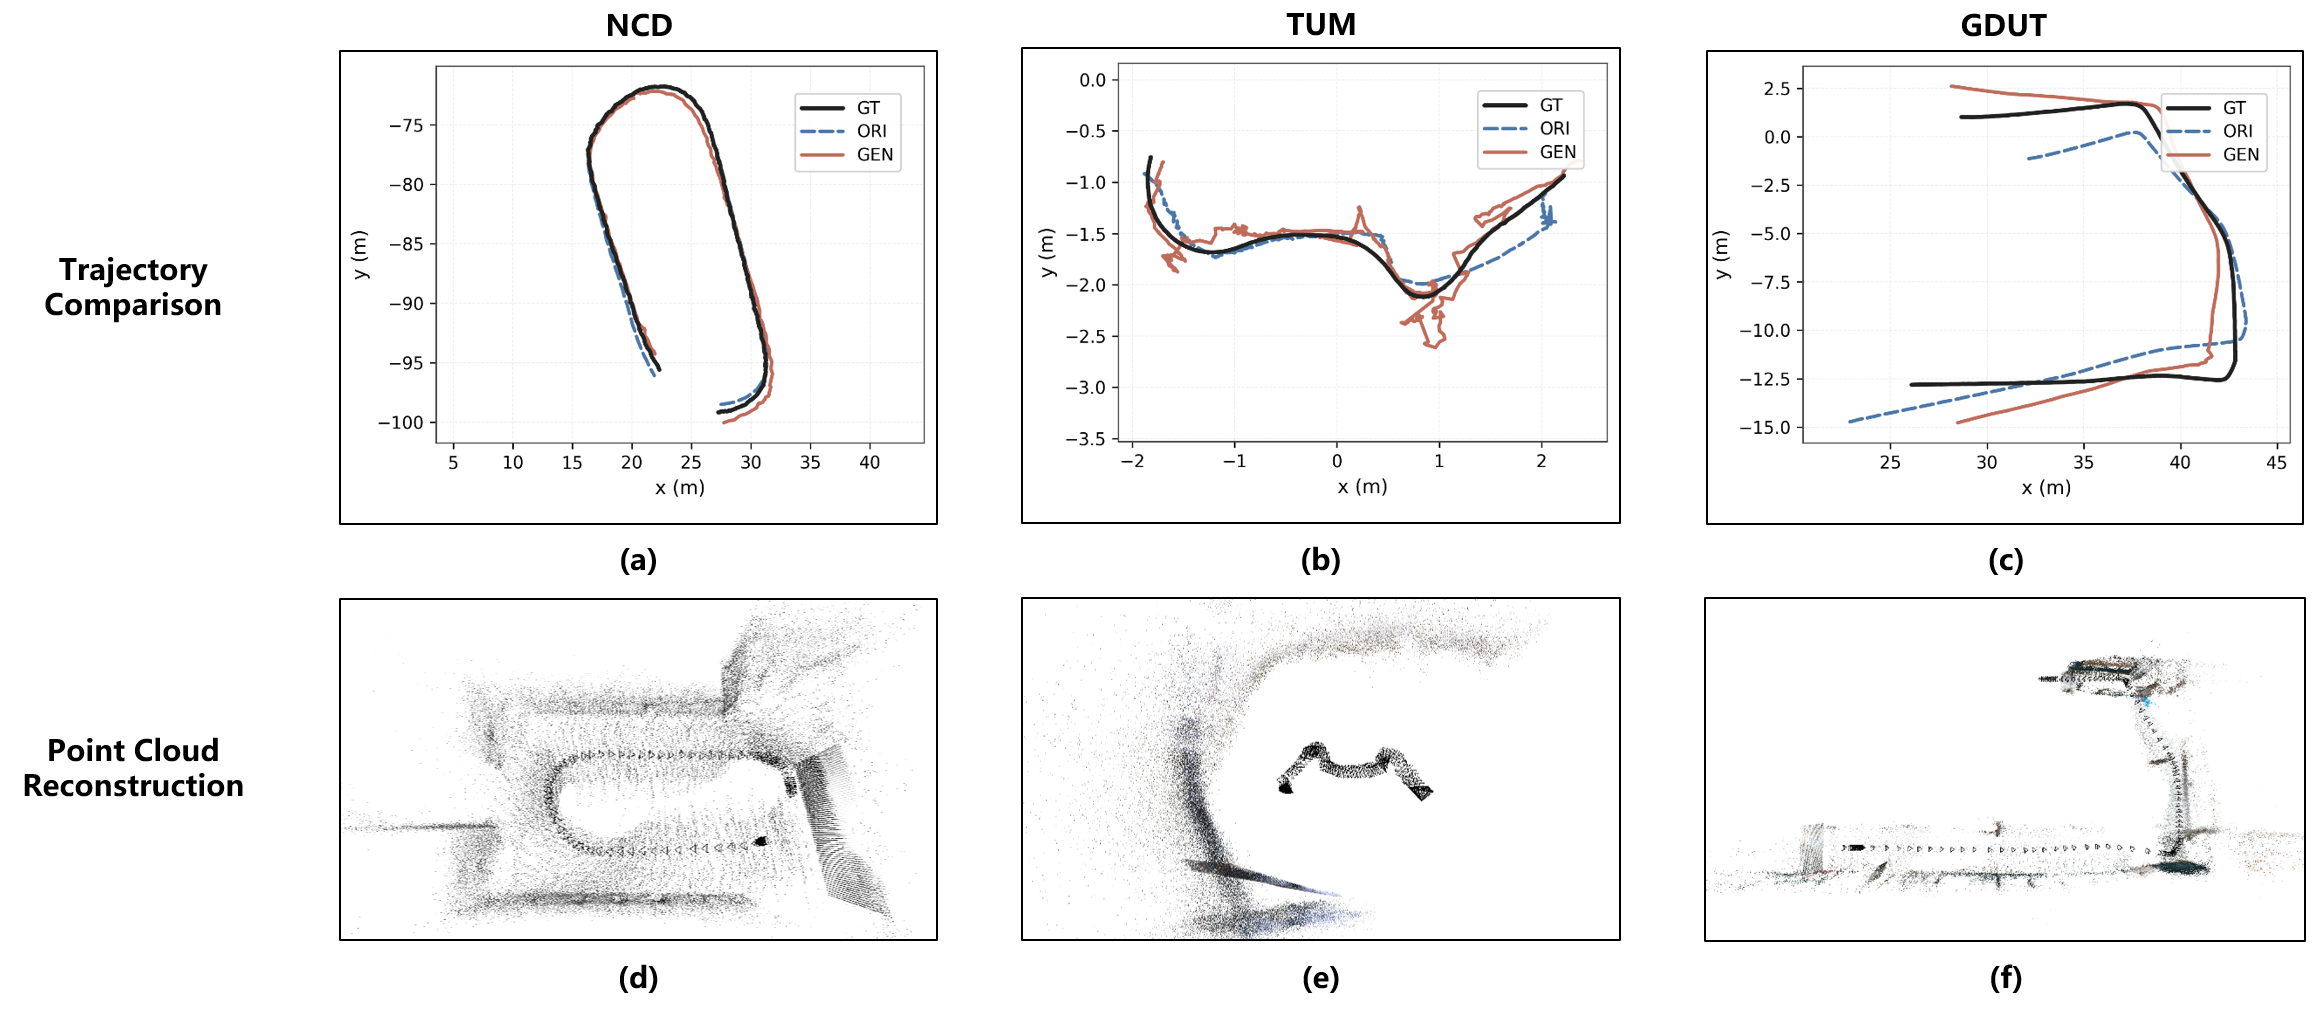
\includegraphics[width=\textwidth]{figures/fig_exp1_trajectory_map.png}
\caption{Trajectory comparison and point-cloud reconstruction results on NCD, TUM, and GDUT.}
\label{fig:trajectory_map}
\end{figure*}

\newpage

Table~\ref{tab:compression_accuracy} reports that, on average, the raw image sequence size is 404.16 MiB, while the transmitted \HVM{} representation is 11.12 MiB. This corresponds to an average data reduction of 96.8\%, indicating that the proposed representation substantially reduces transmitted visual data.

The VSLAM results indicate that this reduction can retain task-usable geometric information. The average ORI APE RMSE is 0.694 m, while the average GEN APE RMSE is 0.707 m. Thus, although GEN APE is close to ORI APE on average, sequence-level differences remain: some generated sequences obtain lower APE than their original counterparts, whereas others obtain higher APE. This behavior is expected because \HVM{} does not aim to reconstruct pixel-identical videos, but to retain enough geometric continuity for downstream VSLAM.

Fig.~\ref{fig:trajectory_map} further illustrates this trend by comparing trajectories and point-cloud reconstructions on NCD, TUM, and GDUT. The generated sequences retain the main route structure and support trackable reconstruction in these examples, which suggests that task-usable geometric continuity can be retained under aggressive transmission reduction.

\subsection{Edge-Side Motion Estimation Benchmark}
\label{subsec:motion_benchmark}

The second experiment compares three edge-side motion estimation choices for constructing motion memory. This benchmark evaluates qualitative segmentation consistency and runtime efficiency, rather than supervised motion-label accuracy.

% This table is included by sections/04_experiments.tex.
\begin{table}[!t]
\renewcommand{\arraystretch}{1.14}
\caption{Runtime comparison of edge-side Motion Response methods.}
\label{tab:motion_benchmark}
\centering
\footnotesize
\setlength{\tabcolsep}{1.5pt}
\begin{tabular*}{\columnwidth}{@{\extracolsep{\fill}}lcccc@{}}
\toprule
Method & Time (s) $\downarrow$ & ms/pair $\downarrow$ & Rel. Cost $\downarrow$ & Valid (\%) $\uparrow$ \\
\midrule
\textbf{Phase Correlation} & \textbf{4.51} & \textbf{4.70} & \textbf{1.00$\times$} & \textbf{100.0} \\
ORB Feature Tracking & 11.73 & 12.22 & 2.60$\times$ & 85.7 \\
Farneback Optical Flow & 29.75 & 30.99 & 6.59$\times$ & 100.0 \\
\bottomrule
\end{tabular*}%
\vspace{0.2em}

\parbox{\columnwidth}{\footnotesize The benchmark is computed on the 40s GDUT clip with 961 frames, corresponding to 960 adjacent frame pairs. Rel. Cost is normalized by PC runtime. Valid ratio denotes the percentage of adjacent frame pairs that produce usable motion evidence.}
\end{table}


\begin{figure*}[!t]
\centering
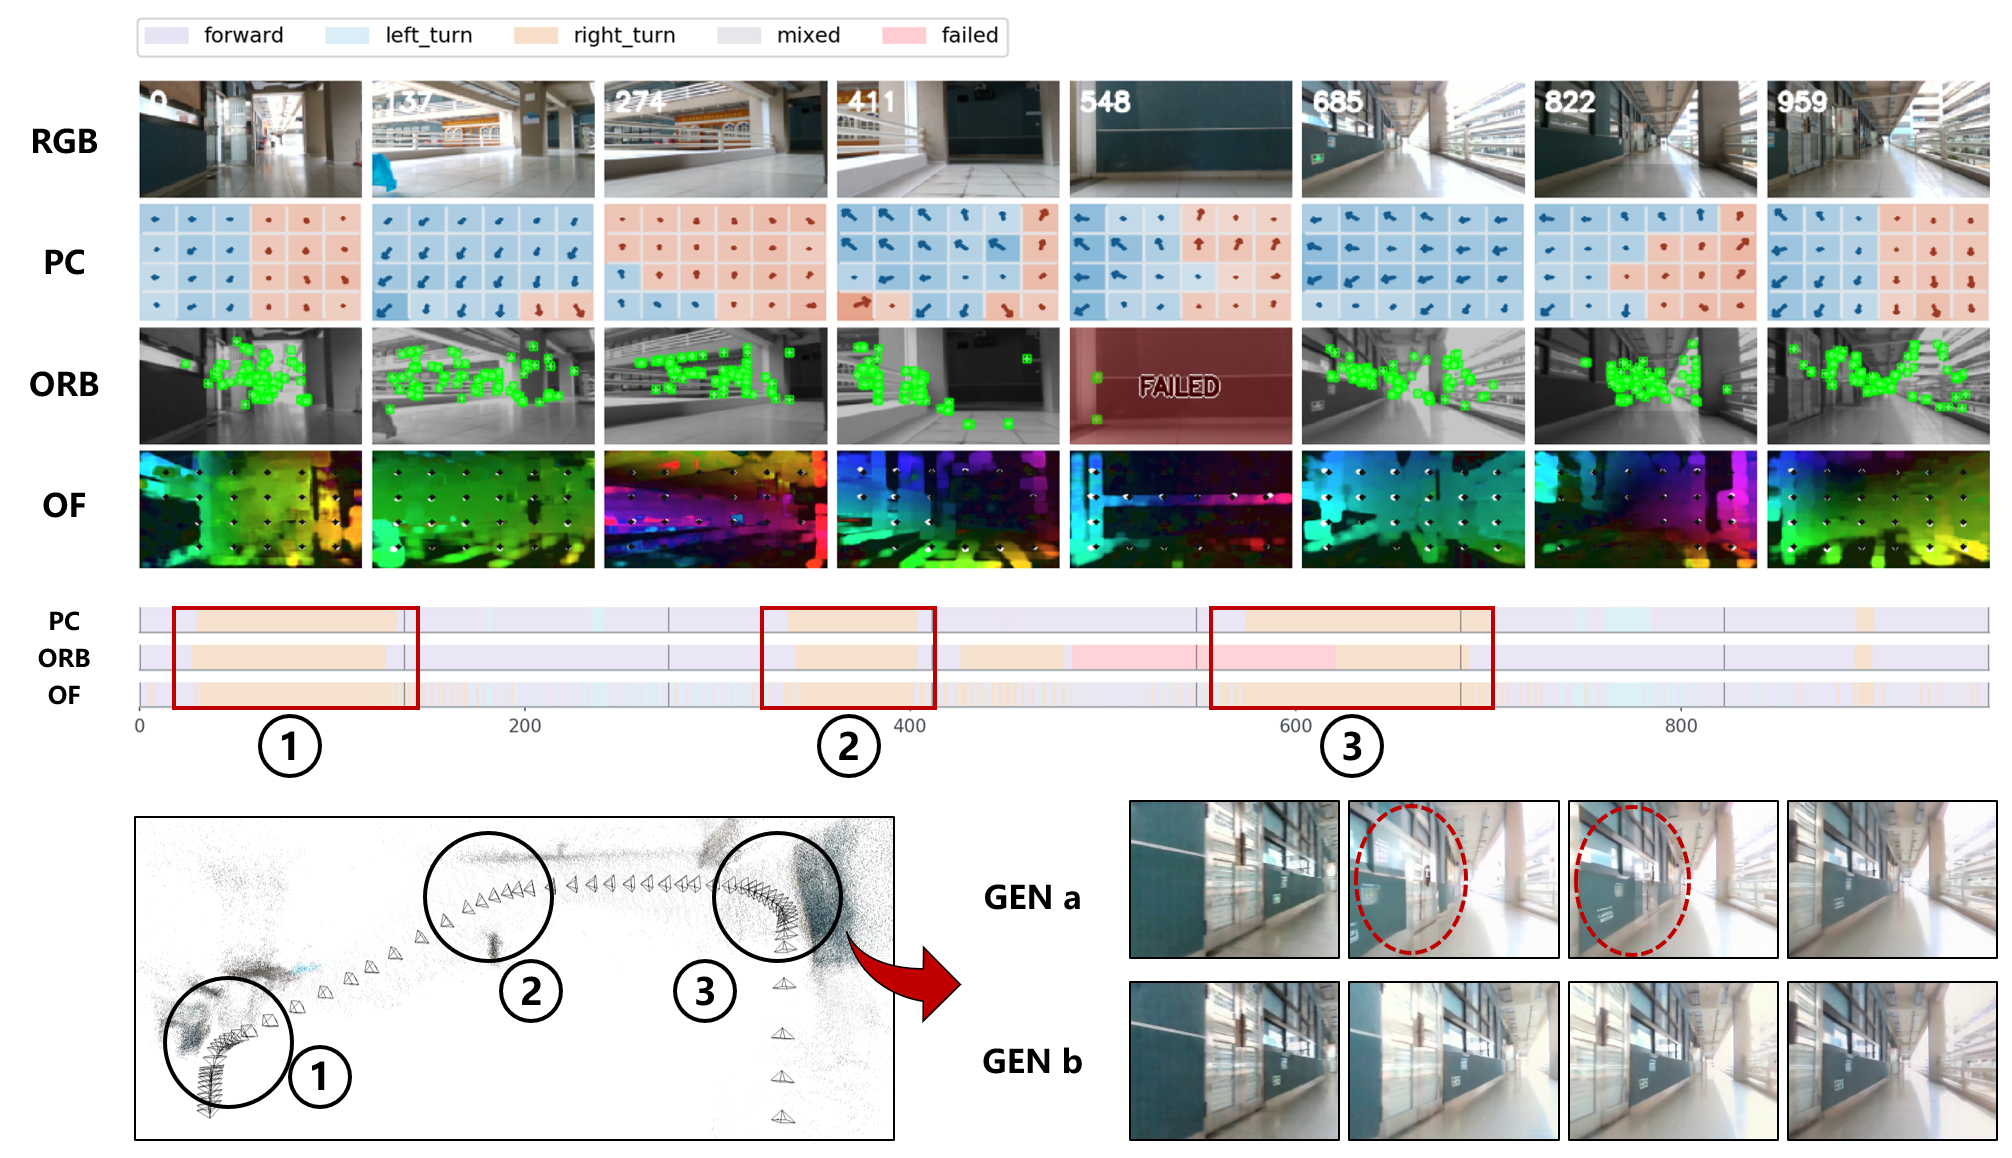
\includegraphics[width=\textwidth]{figures/fig_exp2_motion_benchmark.png}
\caption{Qualitative comparison of phase correlation, ORB feature tracking, and Farneback optical flow for edge-side motion estimation.}
\label{fig:motion_benchmark}
\end{figure*}

\newpage

Fig.~\ref{fig:motion_benchmark} and Table~\ref{tab:motion_benchmark} show the qualitative behavior and runtime cost of the three methods. The valid-output ratio denotes the fraction of frame pairs for which a method produced usable motion evidence.

PC is the lightest option, requiring 4.51 s in total and 4.70 ms per frame pair. ORB feature tracking requires 11.73 s, or 2.60x the PC cost, and produces usable motion evidence for 85.7\% of the evaluated pairs. Farneback optical flow (OF) provides a denser motion field, but its runtime increases to 29.75 s, or 6.59x the PC cost.

These results reflect different edge-side tradeoffs. ORB depends on repeatable local features and can fail in low-texture regions, rapid turns, or tracking-difficult intervals. OF can describe richer local motion but introduces a much higher computational burden. PC provides only coarse global motion, but it can capture language-level trends such as forward motion and turning at the lowest cost, making it suitable as the default edge encoder in \HVM.

\subsection{LoRA Ablation for the World-Model Decoder}
\label{subsec:lora_ablation}

The final experiment ablates the Base and LoRA variants of the world-model decoder.

% This table is included by sections/04_experiments.tex.
\begin{table}[!t]
\renewcommand{\arraystretch}{1.14}
\caption{LoRA ablation results for the world-model decoder.}
\label{tab:lora_ablation}
\centering
\scriptsize
\setlength{\tabcolsep}{2pt}
\begin{tabular*}{\columnwidth}{@{\extracolsep{\fill}}llrrrrr@{}}
\toprule
Data & Dec. & ORI APE & GEN APE & LPIPS & SSIM & FID \\
\midrule
NCD & Base & 0.142 & 0.539 & 0.270 & 0.593 & 50.151 \\
NCD & LoRA & 0.142 & \textbf{0.289} & 0.307 & 0.507 & 23.950 \\
TUM & Base & 0.224 & 0.320 & 0.392 & 0.634 & 71.539 \\
TUM & LoRA & 0.224 & \textbf{0.224} & 0.514 & 0.480 & 104.861 \\
GDUT & Base & 0.354 & 0.968 & 0.345 & 0.587 & 62.169 \\
GDUT & LoRA & 0.354 & \textbf{0.451} & 0.372 & 0.559 & 70.845 \\
Avg. & Base & 0.240 & 0.609 & 0.335 & 0.604 & 61.286 \\
Avg. & LoRA & 0.240 & \textbf{0.321} & 0.398 & 0.515 & 66.552 \\
\bottomrule
\end{tabular*}%
\vspace{0.2em}

\parbox{\columnwidth}{\footnotesize APE values are RMSE in meters. LPIPS, SSIM, and FID are auxiliary image-fidelity metrics and are not the final task-level objective.}
\end{table}


Table~\ref{tab:lora_ablation} shows that the average GEN APE RMSE decreases from 0.609 m with the Base decoder to 0.321 m with LoRA, while the average ORI APE RMSE remains 0.240 m because the original sequences are not affected by the decoder. The same trend appears on NCD, TUM, and GDUT, suggesting that LoRA improves VSLAM-oriented decoding performance across the evaluated data groups.

The image-fidelity metrics do not improve in the same direction. On average, LPIPS changes from 0.335 to 0.398, SSIM changes from 0.604 to 0.515, and FID changes from 61.286 to 66.552. Since LPIPS, SSIM, and FID measure image fidelity and are not the optimization target of \HVM, these changes do not by themselves indicate system failure.

Instead, the ablation indicates that traditional image similarity and VSLAM trajectory quality are not fully aligned in this setting. LoRA appears to bias the decoder toward SLAM-friendly geometry and temporal continuity rather than pixel-level similarity, which supports the task-oriented nature of \HVM.
